% Lab03 — Mineração de métricas DORA. Artigo no template SBC.
% Compilar a partir da raiz do Enunciado 3:
%   uv run python scripts/build_report.py
% O PDF final é copiado para RELATORIO.pdf. Fonte dos números: analysis/output/.
\documentclass[12pt]{article}

\usepackage[utf8]{inputenc}
\usepackage[T1]{fontenc}
\usepackage[brazilian]{babel}
\usepackage{sbc-template}
\renewcommand{\ttdefault}{lmtt} % Courier não vem no TinyTeX; Latin Modern Mono no lugar
\usepackage{graphicx}
\usepackage{url}
\usepackage{booktabs}
\usepackage{tabularx}
\usepackage{multirow}
\usepackage{array}
\usepackage{subcaption}
\usepackage{enumitem}
\usepackage{microtype}
\usepackage[hidelinks]{hyperref}

\graphicspath{{../analysis/output/figures/}}
\setlist{itemsep=1pt,topsep=2pt}
\newcolumntype{Y}{>{\raggedright\arraybackslash}X}
\newcommand{\code}[1]{\texttt{\small #1}}

\sloppy

\title{Mineração de métricas DORA em repositórios open-source:\\
o quanto podemos confiar nos proxies?}

\author{Bernardo Souza Alvim\inst{1}, Luísa Oliveira Jardim\inst{1},
  Pedro Augusto Santos Seabra\inst{1}}

\address{Curso de Engenharia de Software -- Laboratório de Experimentação de Software\\
  Prof. Danilo Maia}

\begin{document}

\maketitle

\begin{abstract}
  We mined the four DORA metrics from 315 popular open-source GitHub
  repositories that use GitHub Actions, over a fixed 12-month window, using
  releases as the deploy proxy and CI runs as the failure proxy. The typical
  repository publishes a release every three weeks, takes about a week from
  commit to release and recovers from CI failures in a few hours. Change
  failure rate depends heavily on the proxy (5.3\% for CI, 42.9\% for
  delivery), and the corrective-release heuristic reached only F1 = 0.57.
  Across repositories, faster delivery
  correlates with more failures; project age is the factor most associated
  with performance. The DORA classification is fairly robust to the
  operational definition (weighted $\kappa$ 0.67--0.84), but not neutral.
\end{abstract}

\begin{resumo}
  Mineramos as quatro métricas DORA de 315 repositórios populares do GitHub
  que usam GitHub Actions, em uma janela fixa de 12 meses, usando releases
  como proxy de deploy e execuções de CI como proxy de falha. O repositório
  típico publica uma release a cada três semanas, leva cerca de uma semana do
  commit à release e se recupera de falhas de CI em poucas horas. A taxa de
  falha depende fortemente do proxy (5,3\% no CI, 42,9\% na entrega), e a
  heurística de release corretiva atingiu só F1 = 0,57. Entre repositórios, entregar mais rápido se
  associa a falhar mais; a idade do projeto é o fator mais associado ao
  desempenho. A classificação DORA é razoavelmente robusta à definição
  operacional ($\kappa$ ponderado 0,67--0,84), mas não neutra.
\end{resumo}

% =====================================================================
\section{Introdução}

As métricas DORA --- \emph{deployment frequency}, \emph{lead time for
changes}, \emph{change failure rate} (CFR) e tempo de recuperação --- se
tornaram o padrão de mercado para medir o desempenho de entrega de software
\cite{forsgren2018,dora2025keys}. Em 2024, o DORA acrescentou uma quinta
métrica, a \emph{deployment rework rate} \cite{dora2024history}. Grande parte
da evidência sobre essas métricas, porém, vem de questionários e de dados de
empresas, o que dificulta comparações abertas e reprodutíveis.

O GitHub não registra ``deploys em produção'' nem ``falhas em produção''.
Este estudo infere as métricas a partir de \emph{proxies}: uma release
publicada faz o papel de deploy, e uma execução de CI com falha faz o papel de
falha. Por isso, além de calcular as métricas, validamos os critérios
automáticos contra o julgamento humano e medimos o quanto as conclusões mudam
quando a definição operacional muda. As questões de pesquisa (RQs) e as
hipóteses informais, escritas antes da coleta, são:

\begin{description}[leftmargin=0pt,font=\normalfont\bfseries]
  \item[RQ01] Qual a frequência de deploys dos repositórios populares que usam
    CI/CD? \emph{Hipótese:} distribuição assimétrica, com a maioria semanal ou
    mensal e poucos projetos diários.
  \item[RQ02] Qual o tempo entre um commit e seu deploy? \emph{Hipótese:} o
    lead time por release (a) terá mediana maior que o lead time por commit
    (b), porque commits antigos ``esquecidos'' inflam (a).
  \item[RQ03] Qual a taxa de falha das mudanças entregues? \emph{Hipóteses:}
    o proxy de CI (a) será maior que o de entrega (b); a heurística de release
    corretiva terá precisão alta ($>$70\%) e recall baixo ($<$50\%).
  \item[RQ04] Qual o tempo de recuperação após uma falha de CI?
    \emph{Hipótese:} repositórios com mais workflow runs recuperam mais rápido.
  \item[RQ05] Quem entrega com mais frequência falha mais ou menos?
    \emph{Hipótese:} correlação fraca a moderada, possivelmente negativa, como
    afirma o DORA.
  \item[RQ06] Que características se associam a melhor desempenho DORA?
    \emph{Hipótese:} bibliotecas e frameworks terão desempenho melhor que
    aplicações e ferramentas CLI.
  \item[RQ07] O quanto a classificação DORA depende da definição operacional?
    \emph{Hipótese:} repositórios Elite serão estáveis, e a fronteira
    Medium/Low mudará com frequência.
  \item[RQ08] (bônus) \emph{Rework rate} e evolução temporal. \emph{Hipótese:}
    mais repositórios com tendência de melhora do que de piora.
\end{description}

% =====================================================================
\section{Metodologia}

\subsection{Fonte de dados, janela e seleção}

A coleta usa um pipeline próprio em Python sobre as APIs REST e GraphQL do
GitHub, sem bibliotecas de acesso à API. A janela de observação vai de
01/10/2025 a 30/09/2026, inclusive. Só entram releases não-draft e
não-pré-release, e workflow runs disparados por \code{push} no
\emph{default branch}, ambos dentro da janela. Um repositório só é incluído
se tiver pelo menos 5 releases e 50 runs válidos na janela. A
Tabela~\ref{tab:funil} resume o funil. A busca foi fatiada em 12 faixas de
estrelas, porque cada consulta devolve no máximo 1.000 resultados. A
população elegível foi congelada em um manifesto de 750 repositórios, do qual
sorteamos a amostra final de 315 com semente fixa (42). A amostra tem de 248
a 42.231 estrelas (mediana 2.881) e de 0,1 a 17,3 anos de idade (mediana
5,9), com predomínio de TypeScript (80), Python (53), Go (47), Rust (29) e
JavaScript (20).

\begin{table}[ht]
  \centering
  \caption{Funil de seleção (gerado pelo estágio \code{report} do pipeline).}
  \label{tab:funil}
  \small
  \begin{tabularx}{\textwidth}{lYr}
    \toprule
    Etapa & Critério & Restantes \\
    \midrule
    Resultados da busca & Search API, 12 faixas de estrelas & 12.000 \\
    Coletados & JSON persistido em \code{data/gold/} & 825 \\
    Elegíveis & $\geq$ 5 releases e $\geq$ 50 runs na janela (64 com poucas releases) & 761 \\
    Manifesto & população congelada (semente 42) & 750 \\
    Amostra final & corte determinístico (semente 42) & 315 \\
    \bottomrule
  \end{tabularx}
\end{table}

\subsection{Definições operacionais}

A Tabela~\ref{tab:defs} resume as definições. Em todas as RQs, a unidade de
análise é o repositório, e reportamos mediana e intervalo interquartil (IQR),
porque as distribuições são muito assimétricas. Os intervalos de confiança
de 95\% das medianas são \emph{bootstrap} BCa com 2.000 reamostragens
\cite{efron1987}.

\begin{table}[ht]
  \centering
  \caption{Definições operacionais das métricas.}
  \label{tab:defs}
  \small
  \begin{tabularx}{\textwidth}{lY}
    \toprule
    Métrica & Definição \\
    \midrule
    Deployment frequency & releases da janela $\div$ 52,1 semanas \\
    Lead time (a) & por release R: \code{published\_at(R)} $-$ data de autoria
      do commit mais antigo em \code{compare/\{anterior\}...\{R\}}; mediana das releases \\
    Lead time (b) & por commit: \code{published\_at(R)} $-$ data de autoria de
      cada commit de R; mediana de todos os commits \\
    CFR (a) & falhas $\div$ (falhas + sucessos) dos runs; falha =
      \code{failure}, \code{timed\_out}, \code{startup\_failure};
      \code{cancelled}, \code{skipped} etc.\ são ignorados \\
    CFR (b) & releases seguidas por uma release corretiva em até 7 dias
      $\div$ releases avaliadas; as dos últimos 7 dias da janela são censuradas \\
    Recuperação & por workflow: da 1ª falha após um sucesso
      (\code{run\_started\_at}) até o próximo sucesso (\code{updated\_at});
      mediana dos episódios; episódios sem sucesso na janela são censurados \\
    \emph{Rework rate} & releases corretivas $\div$ releases da janela,
      com a mesma heurística da CFR (b) \\
    \bottomrule
  \end{tabularx}
\end{table}

Para a classificação DORA, cada métrica recebe 4 (Elite), 3 (High), 2
(Medium) ou 1 (Low) ponto, pelos cortes fixos da disciplina, e a categoria
geral é a mediana das quatro notas, arredondada para baixo. Na RQ07,
comparamos três combinações: C1 (release, lead time (a), CFR (a)), C2
(release + tags, lead time (a), CFR (a)) e C3 (release + tags, lead time (b),
CFR (a)). O CFR (a) foi mantido nas três porque, com F1 = 0,57, uma variante
com CFR (b) mediria sobretudo o erro da heurística. Pré-releases não viraram
variante: são 14,7\% das releases da janela, e 74\% dos repositórios não
publicam nenhuma.

\subsection{Validação manual (amostra-ouro)}

Sorteamos 60 repositórios da amostra final (semente 42) e 5 releases de cada.
Três avaliadores rotularam, de forma independente e sem ver a saída da
heurística, o tipo do projeto, se as releases representam entregas reais e
se cada release é corretiva. Para isso, usaram dossiês gerados
automaticamente com notas de release, commits e links. Um dos três
avaliadores foi um modelo de linguagem (Claude), declarado no protocolo. A
concordância foi medida com o $\kappa$ de Fleiss \cite{fleiss1971}, e o
consenso foi definido por maioria simples, com empates 1-1-1 decididos em
reunião. A heurística de release corretiva passou por quatro versões,
avaliadas por precisão, recall e F1 contra o consenso:
\begin{itemize}
  \item v1: só o PATCH do SemVer mudou;
  \item v2: v1 ou commit com \code{fix}, \code{revert} ou \code{hotfix};
  \item v3: pontuação ponderada com corte;
  \item v4: $1\cdot(\mbox{PATCH}>0) + 2\cdot{}$fração de commits com
    palavra-chave $\geq 0{,}75$.
\end{itemize}
Um laço automático testou 197 combinações de palavras-chave, tipo de
casamento, corte e penalidade para commits \code{feat}. O F1 fora da amostra
foi estimado por validação cruzada 5-fold por repositório, com 20 repetições.

\subsection{Análise estatística e inovações do grupo}

A RQ05 usa a correlação de Spearman com IC BCa pareado. A RQ06 usa
Kruskal-Wallis \cite{kruskal1952} para quatro fatores (linguagem, quartis de
estrelas, quartis de idade e tipo do projeto) e cinco métricas, com correção
de Holm \cite{holm1979} sobre os 20 testes e tamanho de efeito
$\varepsilon^2 = H/(n-1)$ \cite{rea1992}. A RQ07 usa o $\kappa$ de Cohen
ponderado linear \cite{cohen1968}, e a RQ08 usa o teste de Mann-Kendall
\cite{mann1945}. Além do exigido, o grupo propôs:
\begin{enumerate}[label=(\roman*)]
  \item curva de Kaplan-Meier \cite{kaplan1958} para a recuperação censurada,
    e IC BCa para todas as medianas;
  \item \emph{post-hoc} de Dunn \cite{dunn1964} com Holm e $\delta$ de Cliff
    \cite{romano2006} na RQ06;
  \item as duas opções do bônus da RQ08, com Mann-Kendall também em escala
    mensal;
  \item arquitetura de coleta com cache SQLite, retomada, pool de tokens e
    GraphQL em lote;
  \item reprodução exata do estudo sem token, a partir do manifesto e dos
    JSONs versionados.
\end{enumerate}

% =====================================================================
\section{Resultados}

A Tabela~\ref{tab:desc} resume as métricas das RQ01 a RQ04. As ausências
são estruturais. Das 13.270 releases da janela, 62,6\% entram no lead time;
21,1\% não têm commits novos, 15,8\% foram ignoradas porque o \code{compare}
retornou 404 (tag apagada ou reescrita) e 0,5\% não têm release anterior.
Isso deixa 43 repositórios sem lead time. Outros 30 não têm tempo de
recuperação, por não terem nenhum episódio de falha encerrado.

\begin{table}[ht]
  \centering
  \caption{Estatística descritiva por repositório (IC 95\% BCa da mediana).}
  \label{tab:desc}
  \small
  \begin{tabular}{llrrcc}
    \toprule
    RQ & Métrica & n & Mediana & IQR (Q1--Q3) & IC 95\% \\
    \midrule
    RQ01 & Deployment frequency (releases/semana) & 315 & 0,35 & 0,19--0,77 & 0,31--0,40 \\
    RQ02 & Lead time (a), por release (h) & 272 & 166,3 & 22,7--626,0 & 118,5--247,7 \\
         & Lead time (b), por commit (h) & 272 & 151,7 & 24,8--404,3 & 120,1--187,8 \\
    RQ03 & CFR (a), proxy de CI & 315 & 0,053 & 0,020--0,116 & 0,043--0,064 \\
         & CFR (b), proxy de entrega & 315 & 0,429 & 0,167--0,710 & --- \\
    RQ04 & Tempo de recuperação (h) & 285 & 3,32 & 0,63--17,71 & 2,38--4,89 \\
    \bottomrule
  \end{tabular}
\end{table}

\textbf{Amostra-ouro.} A concordância entre os três avaliadores foi quase
perfeita para o tipo do projeto ($\kappa = 0{,}95$) e moderada para
``entrega ao usuário'' ($\kappa = 0{,}49$) e para ``release corretiva''
($\kappa = 0{,}60$) \cite{landis1977}. Em ``entrega'', 59 dos 60 itens foram
unânimes, mas quase todos são ``sim'', e esse desbalanceamento derruba o
$\kappa$. Em ``corretiva'', 70\% das releases foram unânimes. A melhor
heurística foi a v4 (precisão 0,44; recall 0,84; F1 0,57; 0,53 em validação
cruzada). As outras versões ficaram próximas: v1 0,53, v2 0,54 e v3 0,56.
Nenhuma atingiu a meta de F1 $\geq$ 0,70 do enunciado.

\textbf{RQ01.} A mediana é de 0,35 release por semana, cerca de uma a cada
três semanas. 28\% dos repositórios publicam menos de uma release por mês,
17,5\% publicam semanalmente ou mais, e só 3 atingem frequência diária. Na
classificação geral C1, predominam High (35,9\%) e Medium (30,8\%), com 7,0\%
Elite, 4,4\% Low e 21,9\% não classificáveis (Figura~\ref{fig:rq01}).

\begin{figure}[ht]
  \centering
  \begin{subfigure}{0.49\textwidth}
    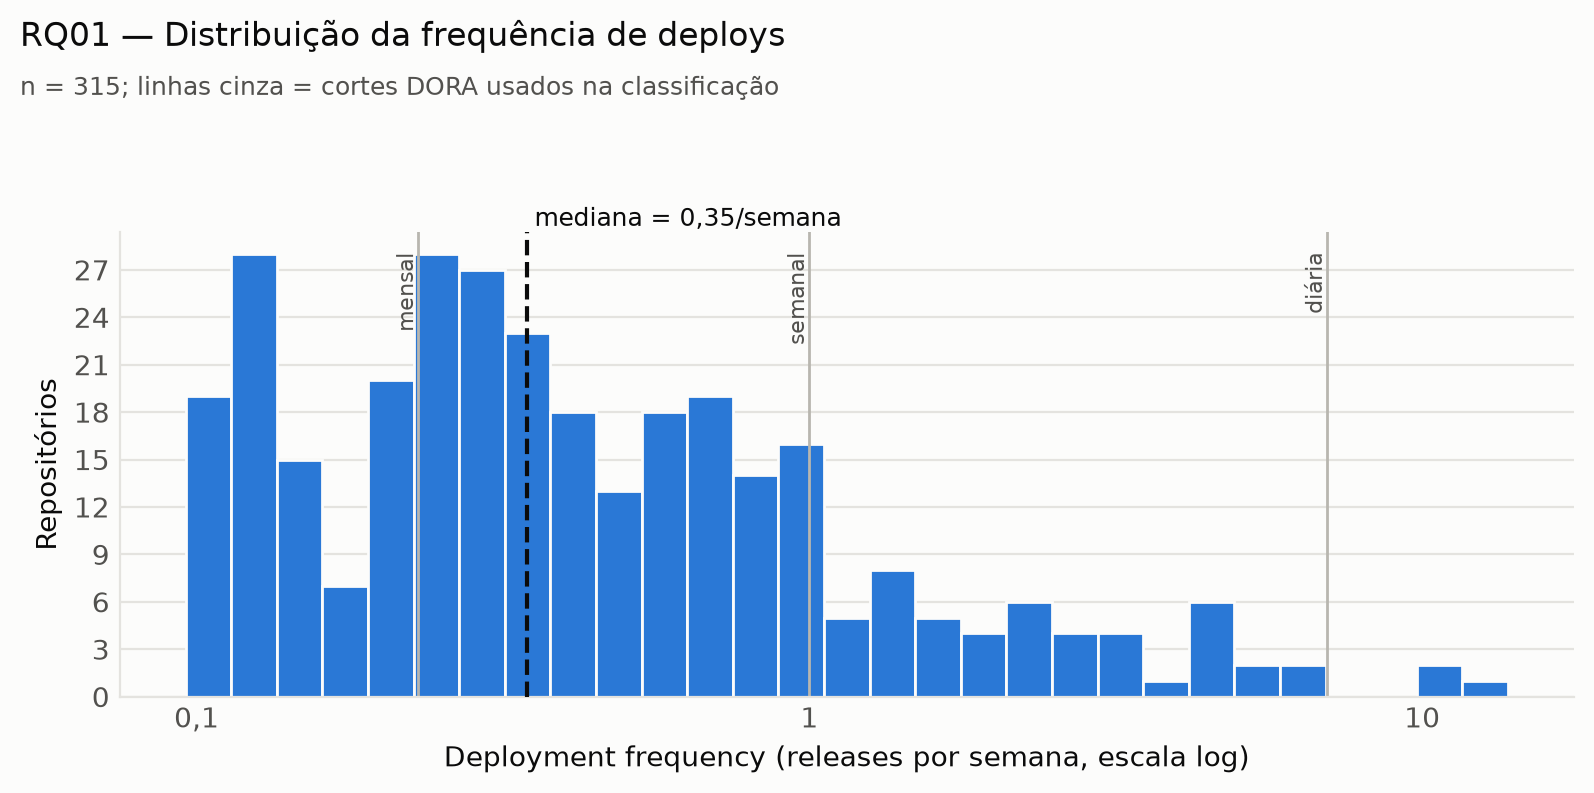
\includegraphics[width=\linewidth]{fig02_rq01_deploy_freq.png}
    \caption{Deployment frequency.}
  \end{subfigure}\hfill
  \begin{subfigure}{0.49\textwidth}
    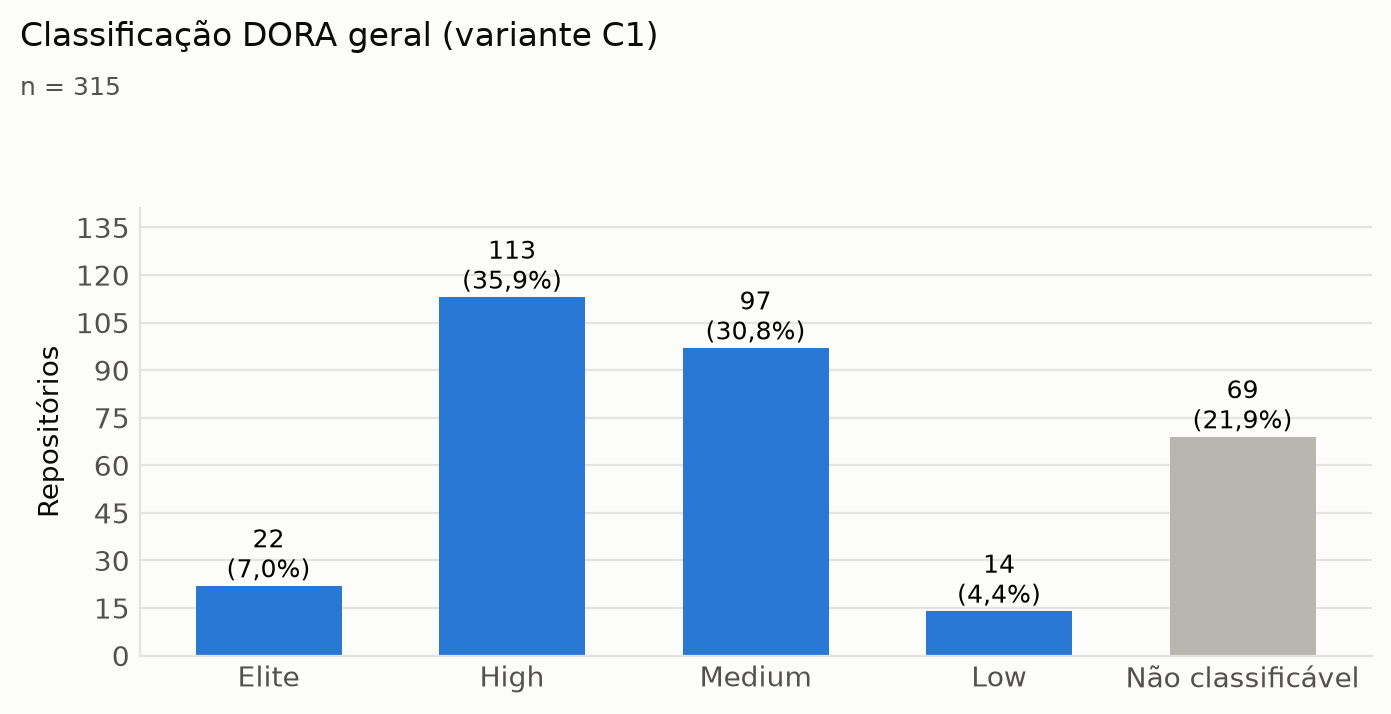
\includegraphics[width=\linewidth]{fig03_rq01_dora_c1.png}
    \caption{Classificação DORA (C1).}
  \end{subfigure}
  \caption{RQ01: frequência de deploy e classificação geral.}
  \label{fig:rq01}
\end{figure}

\textbf{RQ02 e RQ03.} O lead time mediano é de 166~h ($\approx$ 7 dias) na
variante (a) e de 152~h ($\approx$ 6,3 dias) na (b). A variante (a) é maior
em 69\% dos repositórios e tem IQR bem maior (603~h contra 380~h). Os dois
proxies de falha contam histórias diferentes (Figura~\ref{fig:rq0203}). No CI
(a), a mediana é de 5,3\% de runs com falha, e 80\% dos repositórios ficam
no corte Elite ($\leq$ 15\%). Na entrega (b), a mediana é de 42,9\%, e só
22,5\% ficam abaixo de 15\%.

\begin{figure}[ht]
  \centering
  \begin{subfigure}{0.49\textwidth}
    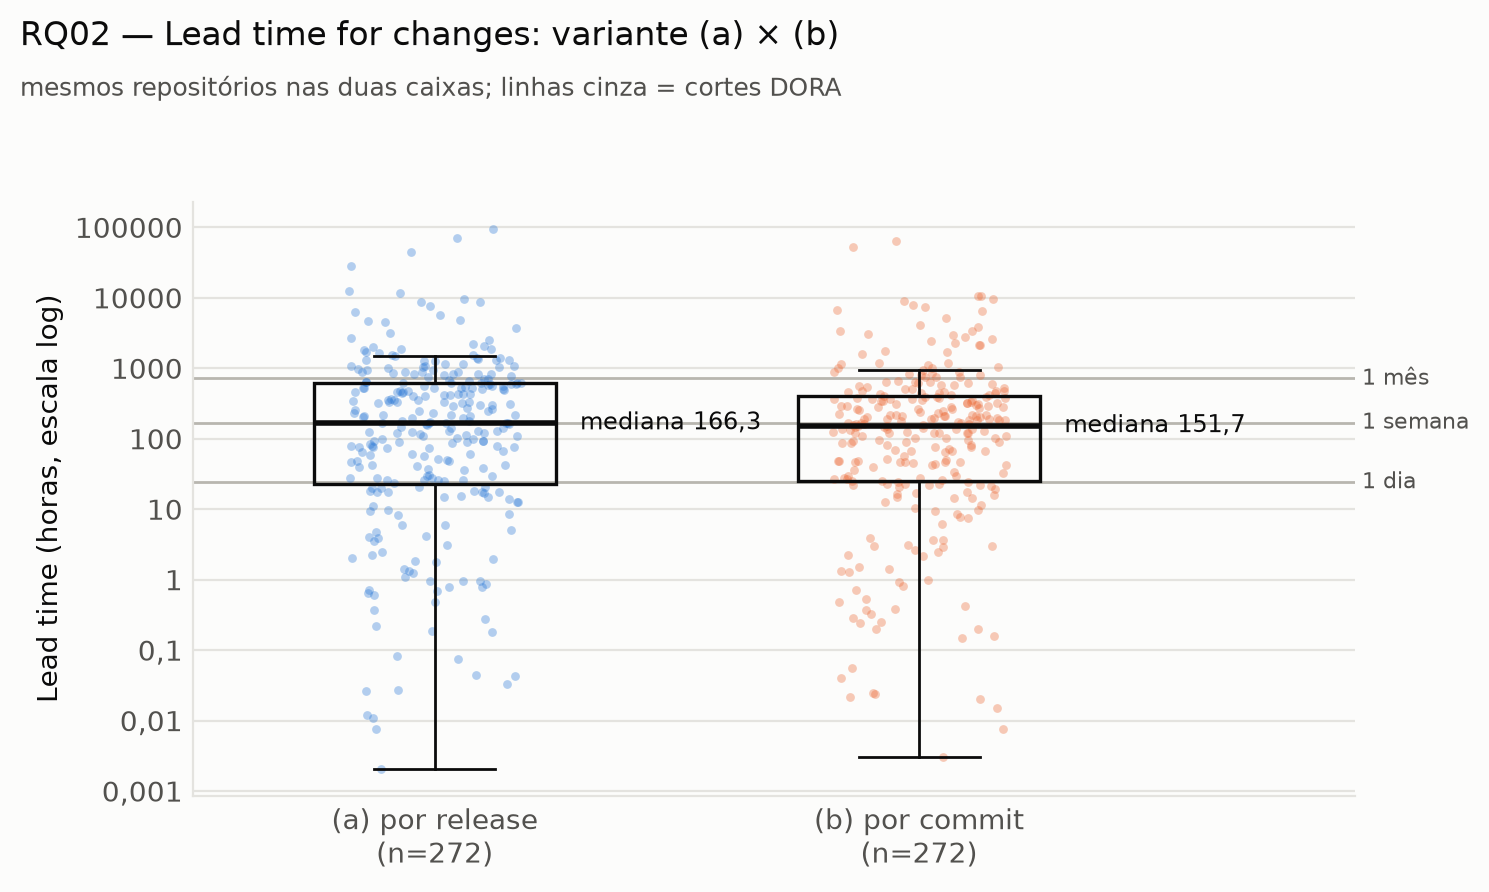
\includegraphics[width=\linewidth]{fig04_rq02_lead_time.png}
    \caption{RQ02: lead time (a) $\times$ (b).}
  \end{subfigure}\hfill
  \begin{subfigure}{0.49\textwidth}
    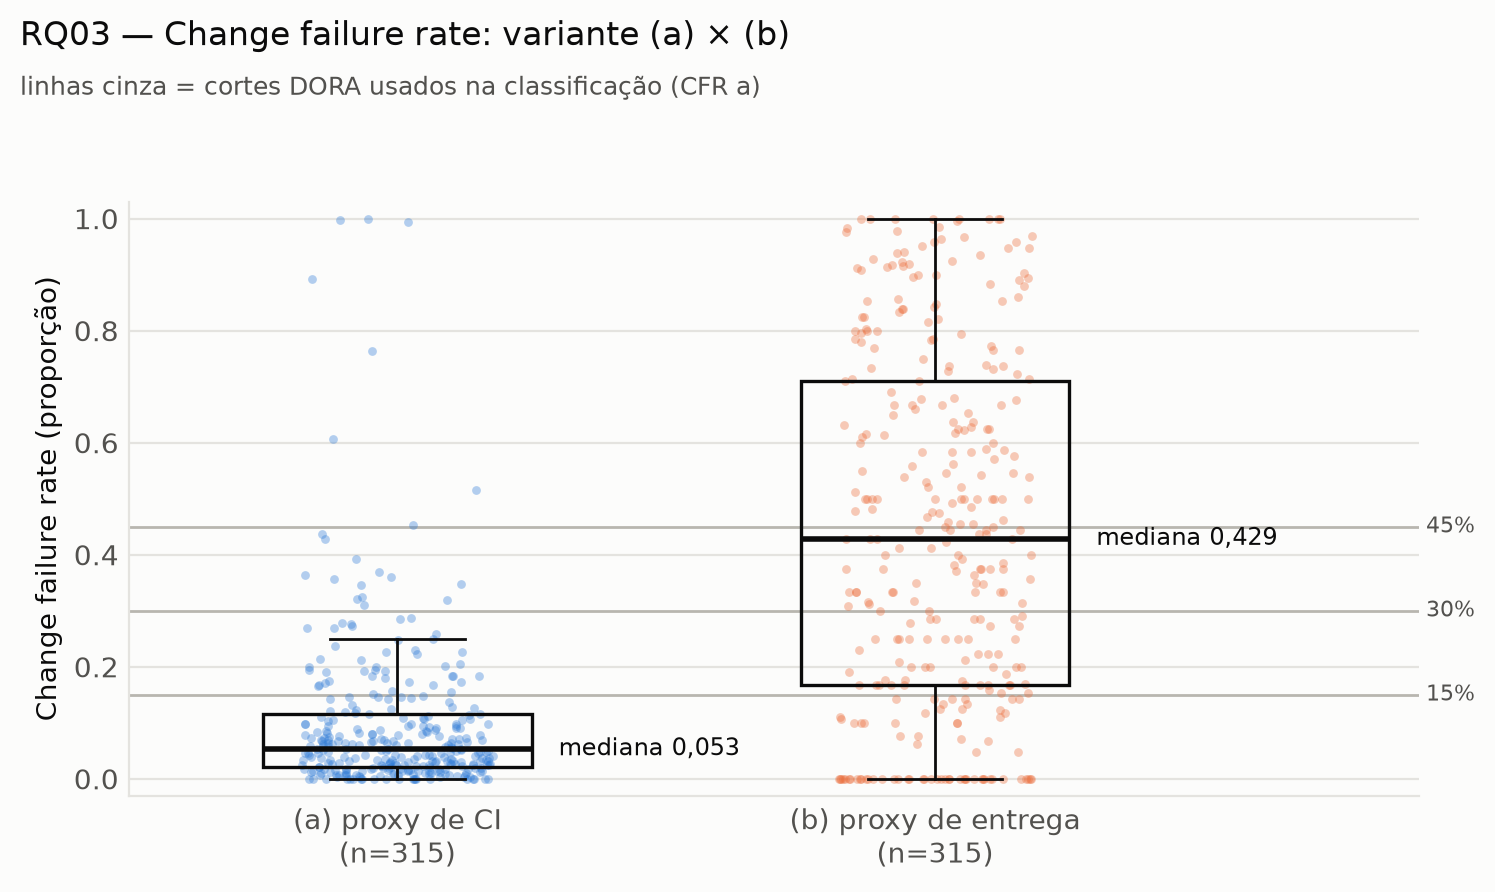
\includegraphics[width=\linewidth]{fig05_rq03_cfr.png}
    \caption{RQ03: CFR (a) $\times$ (b).}
  \end{subfigure}
  \caption{Lead time e taxa de falha (escala log; linhas cinza = cortes DORA).}
  \label{fig:rq0203}
\end{figure}

\textbf{RQ04.} A recuperação mediana por repositório é de 3,3~h: 31\% dos
repositórios recuperam em menos de 1 hora e 81\% em menos de 1 dia. Foram
7.062 episódios, dos quais 76 (1,1\%) ficaram censurados. Com eles, a curva
de Kaplan-Meier dá uma mediana de 4,4~h (Figura~\ref{fig:rq04}). O número de
runs válidos (mediana 323 por repositório) não tem relação com a
recuperação ($\rho = 0{,}01$; IC 95\% $-0{,}11$ a $0{,}13$; $p = 0{,}87$;
$n = 285$).

\begin{figure}[ht]
  \centering
  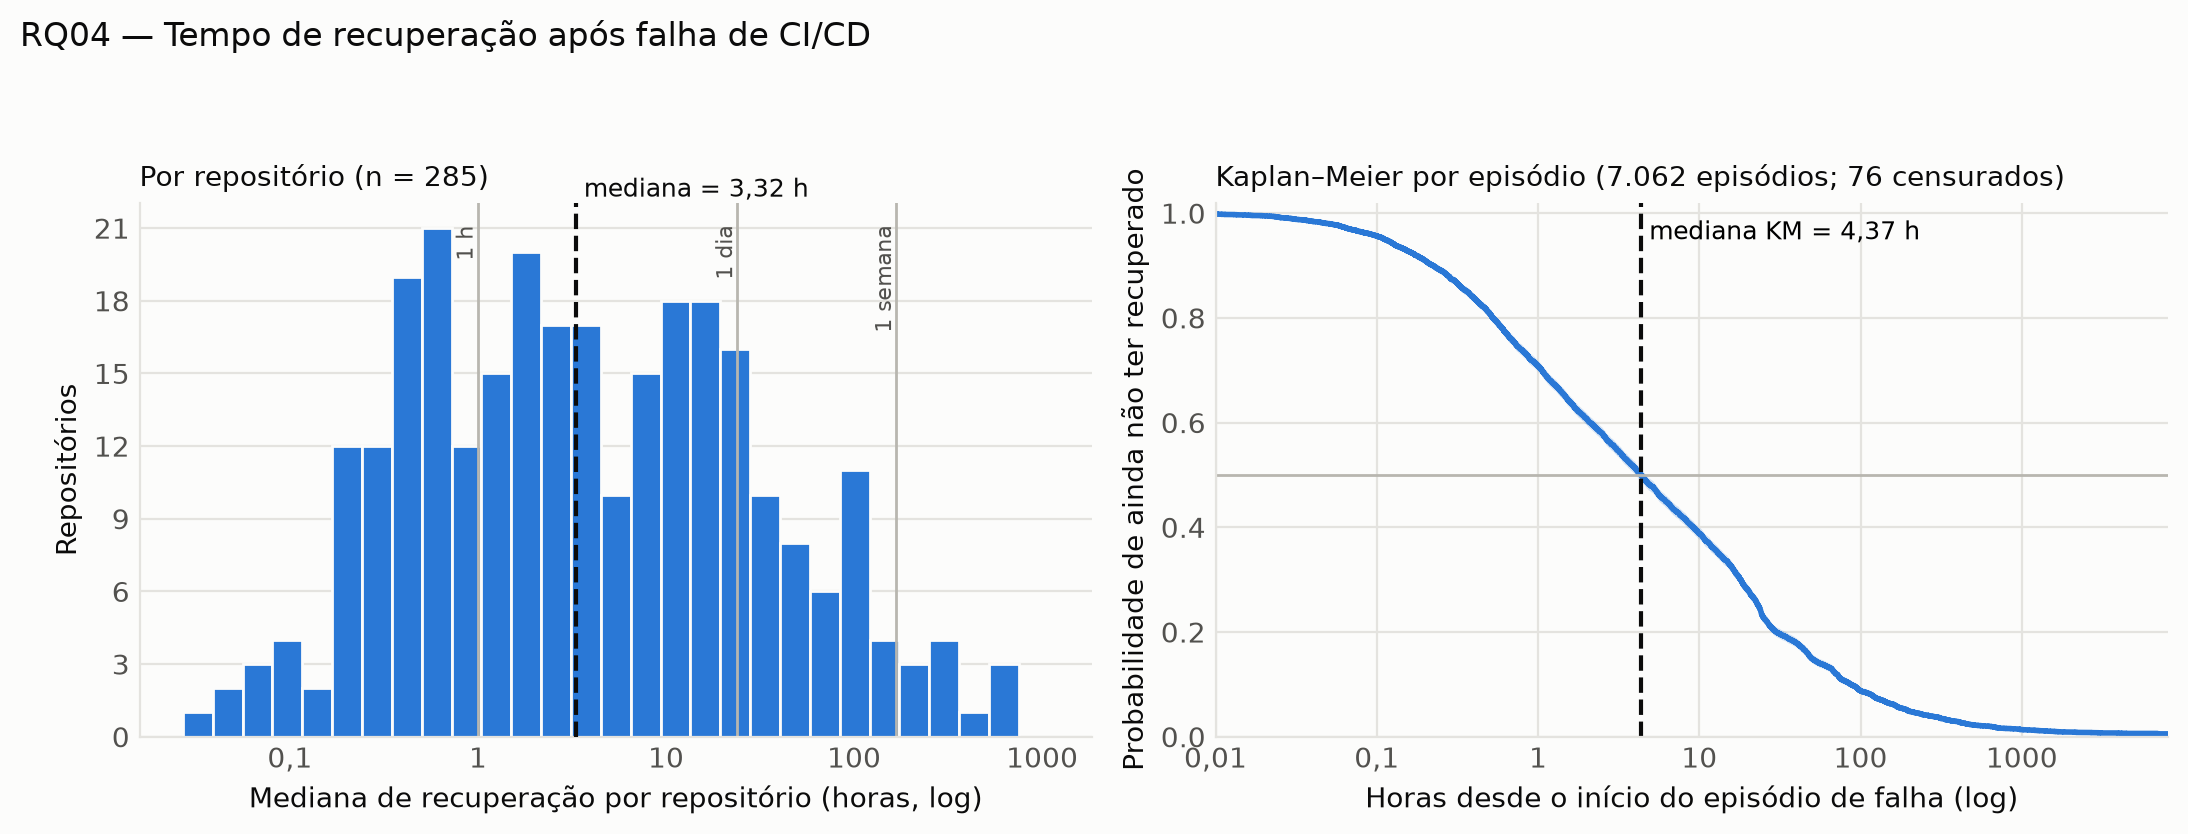
\includegraphics[width=0.82\textwidth]{fig06_rq04_recovery.png}
  \caption{RQ04: recuperação por repositório e curva de Kaplan-Meier dos episódios.}
  \label{fig:rq04}
\end{figure}

\textbf{RQ05.} A correlação de Spearman entre frequência de deploy e taxa de
falha é positiva nas duas variantes (Figura~\ref{fig:rq05}). Ela é fraca no
CFR (a) ($\rho = 0{,}13$; IC 95\% 0,02--0,25; $p = 0{,}018$) e forte no CFR
(b) ($\rho = 0{,}69$; IC 95\% 0,61--0,75; $p < 0{,}001$), com $n = 315$ nas
duas.

\begin{figure}[ht]
  \centering
  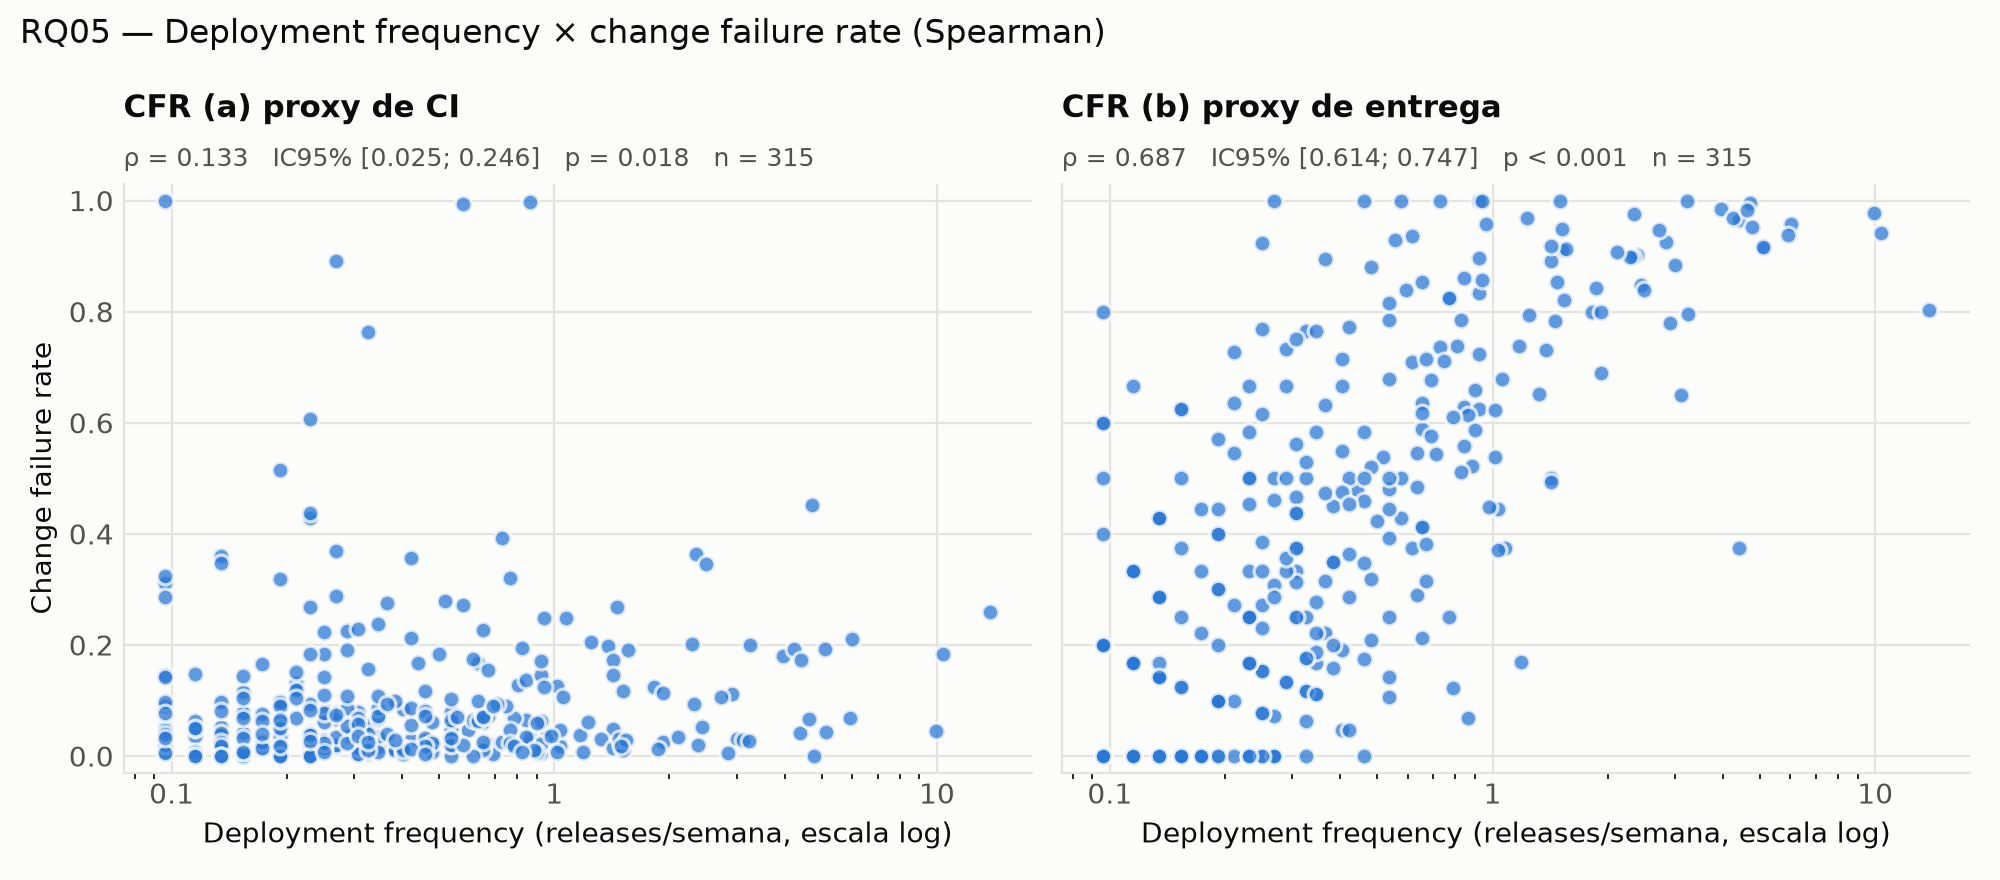
\includegraphics[width=0.78\textwidth]{rq05_scatter.png}
  \caption{RQ05: deployment frequency (escala log) $\times$ CFR (a) e (b).}
  \label{fig:rq05}
\end{figure}

\textbf{RQ06.} Dos 20 testes de Kruskal-Wallis, 7 são significativos após
Holm (Figura~\ref{fig:rq06}a). A idade é o fator dominante: tem efeito em
deployment frequency ($\varepsilon^2 = 0{,}12$), lead time (0,27), CFR (b)
(0,24) e recuperação (0,06). Pelo \emph{post-hoc} de Dunn, o quartil mais
jovem publica mais (0,61 contra 0,25 release/semana no mais antigo;
$\delta = 0{,}56$), tem lead time muito menor (18~h contra 556~h;
$\delta = -0{,}75$) e recupera mais rápido (1,5~h contra 10,8~h;
$\delta = -0{,}35$). Em contrapartida, tem CFR (b) muito maior (0,77 contra
0,25; $\delta = 0{,}73$) (Figura~\ref{fig:rq06}b). A linguagem tem efeito
moderado em frequência, lead time e CFR (b): TypeScript, por exemplo, tem lead
time menor que Go (73~h contra 315~h). Popularidade e tipo do projeto não têm
efeito significativo. O tipo, porém, só existe para os 55 repositórios
rotulados da amostra-ouro.

\begin{figure}[ht]
  \centering
  \begin{subfigure}{0.40\textwidth}
    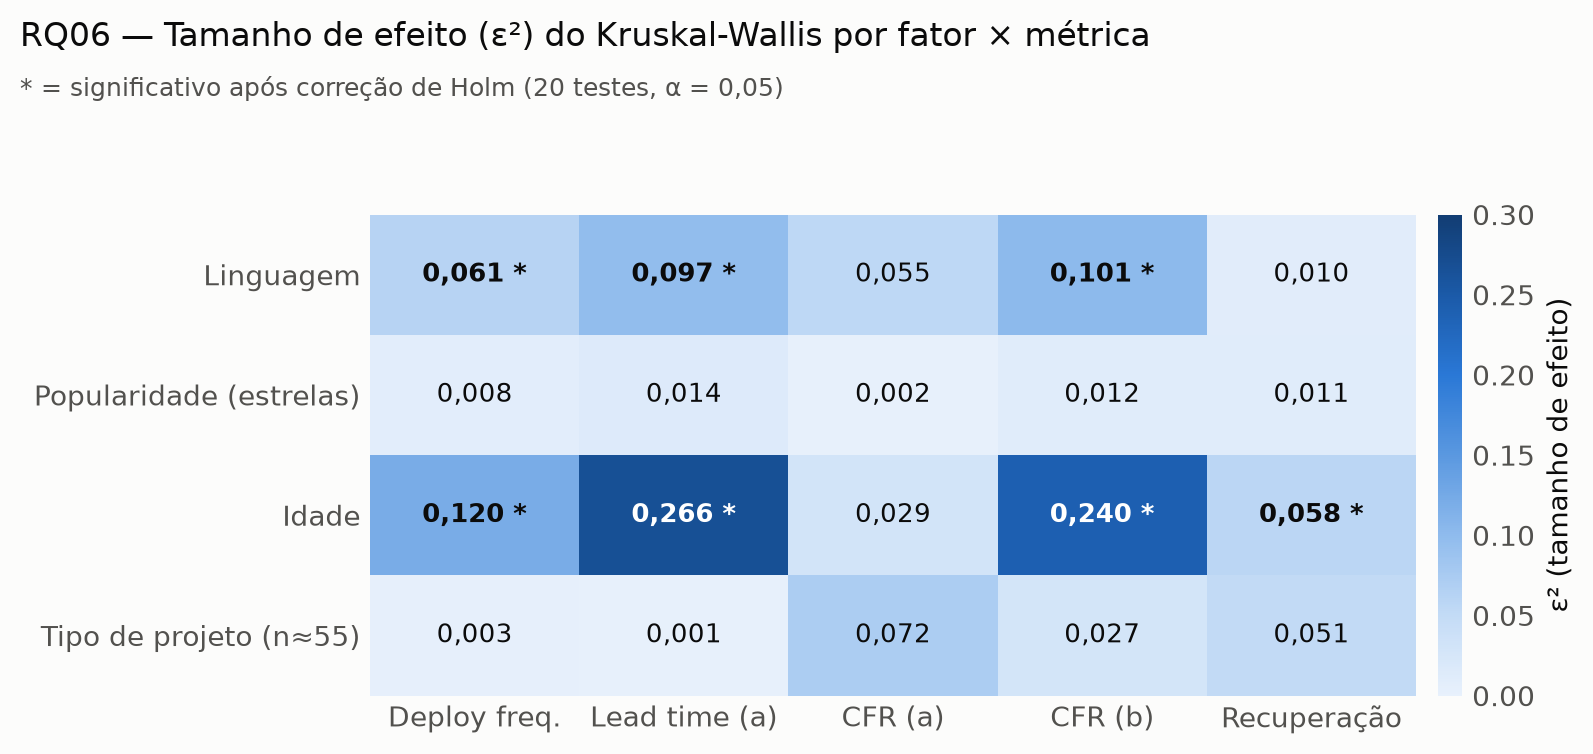
\includegraphics[width=\linewidth]{fig07_rq06_heatmap.png}
    \caption{$\varepsilon^2$ por fator $\times$ métrica.}
  \end{subfigure}\hfill
  \begin{subfigure}{0.58\textwidth}
    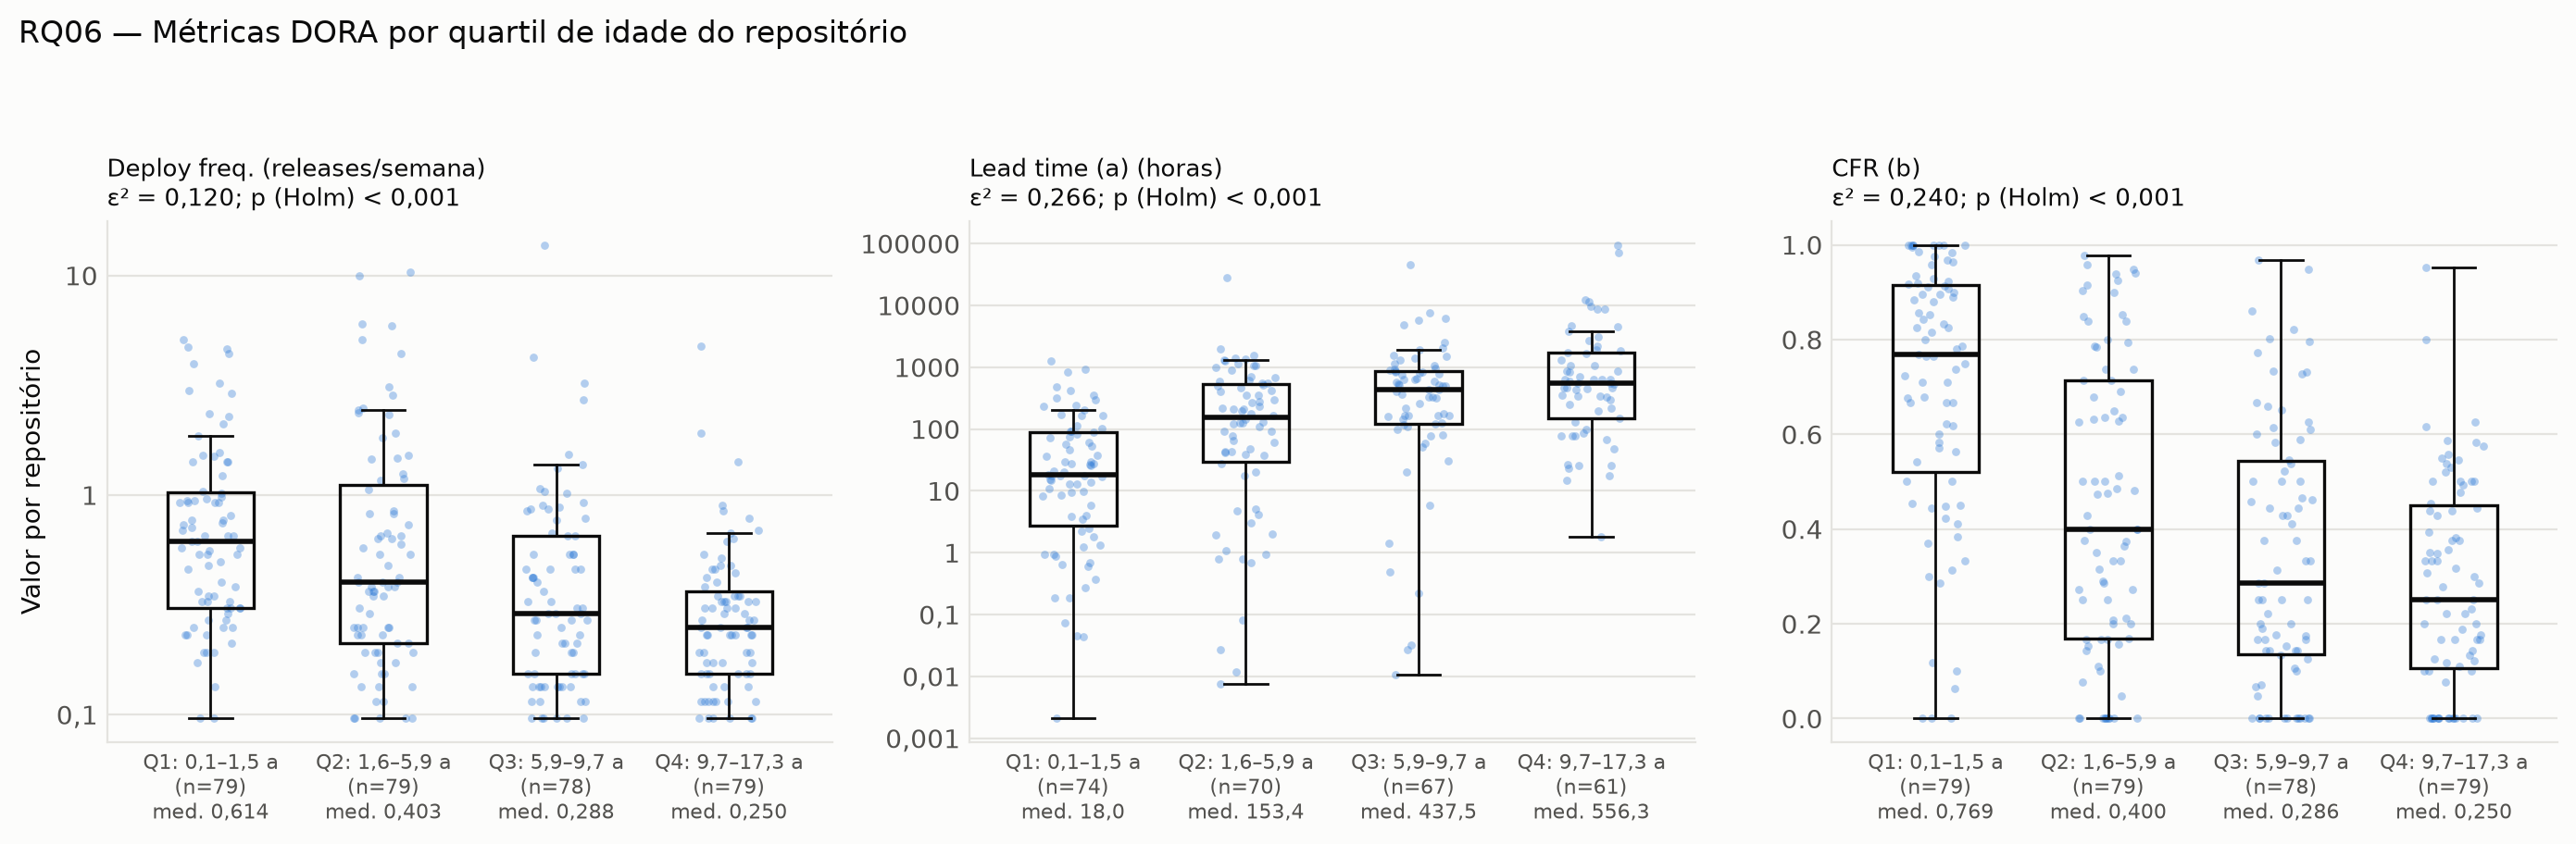
\includegraphics[width=\linewidth]{fig08_rq06_idade.png}
    \caption{Métricas por quartil de idade.}
  \end{subfigure}
  \caption{RQ06: características associadas ao desempenho DORA.}
  \label{fig:rq06}
\end{figure}

\textbf{RQ07.} Entre os 246 repositórios classificáveis nas três variantes, a
categoria muda em 14,6\% entre C1 e C2, em 23,6\% entre C1 e C3 e em 11,0\%
entre C2 e C3 (Tabela~\ref{tab:rq07}). Contar tags como deploy (C1 $\to$ C2)
só melhora categorias: 36 repositórios sobem, nenhum desce, e a categoria Low
cai de 14 para 6. Só um repositório salta dois níveis (Figura~\ref{fig:rq07}).

\begin{table}[ht]
  \centering
  \caption{RQ07: mudança de categoria e concordância entre variantes ($n = 246$).}
  \label{tab:rq07}
  \small
  \begin{tabular}{lrrrc}
    \toprule
    Par & Mudaram & Melhoraram & Pioraram & $\kappa$ linear \\
    \midrule
    C1 $\times$ C2 & 14,6\% & 36 & 0 & 0,80 (quase perfeita) \\
    C1 $\times$ C3 & 23,6\% & 47 & 11 & 0,67 (substancial) \\
    C2 $\times$ C3 & 11,0\% & 14 & 13 & 0,84 (quase perfeita) \\
    \bottomrule
  \end{tabular}
\end{table}

\begin{figure}[ht]
  \centering
  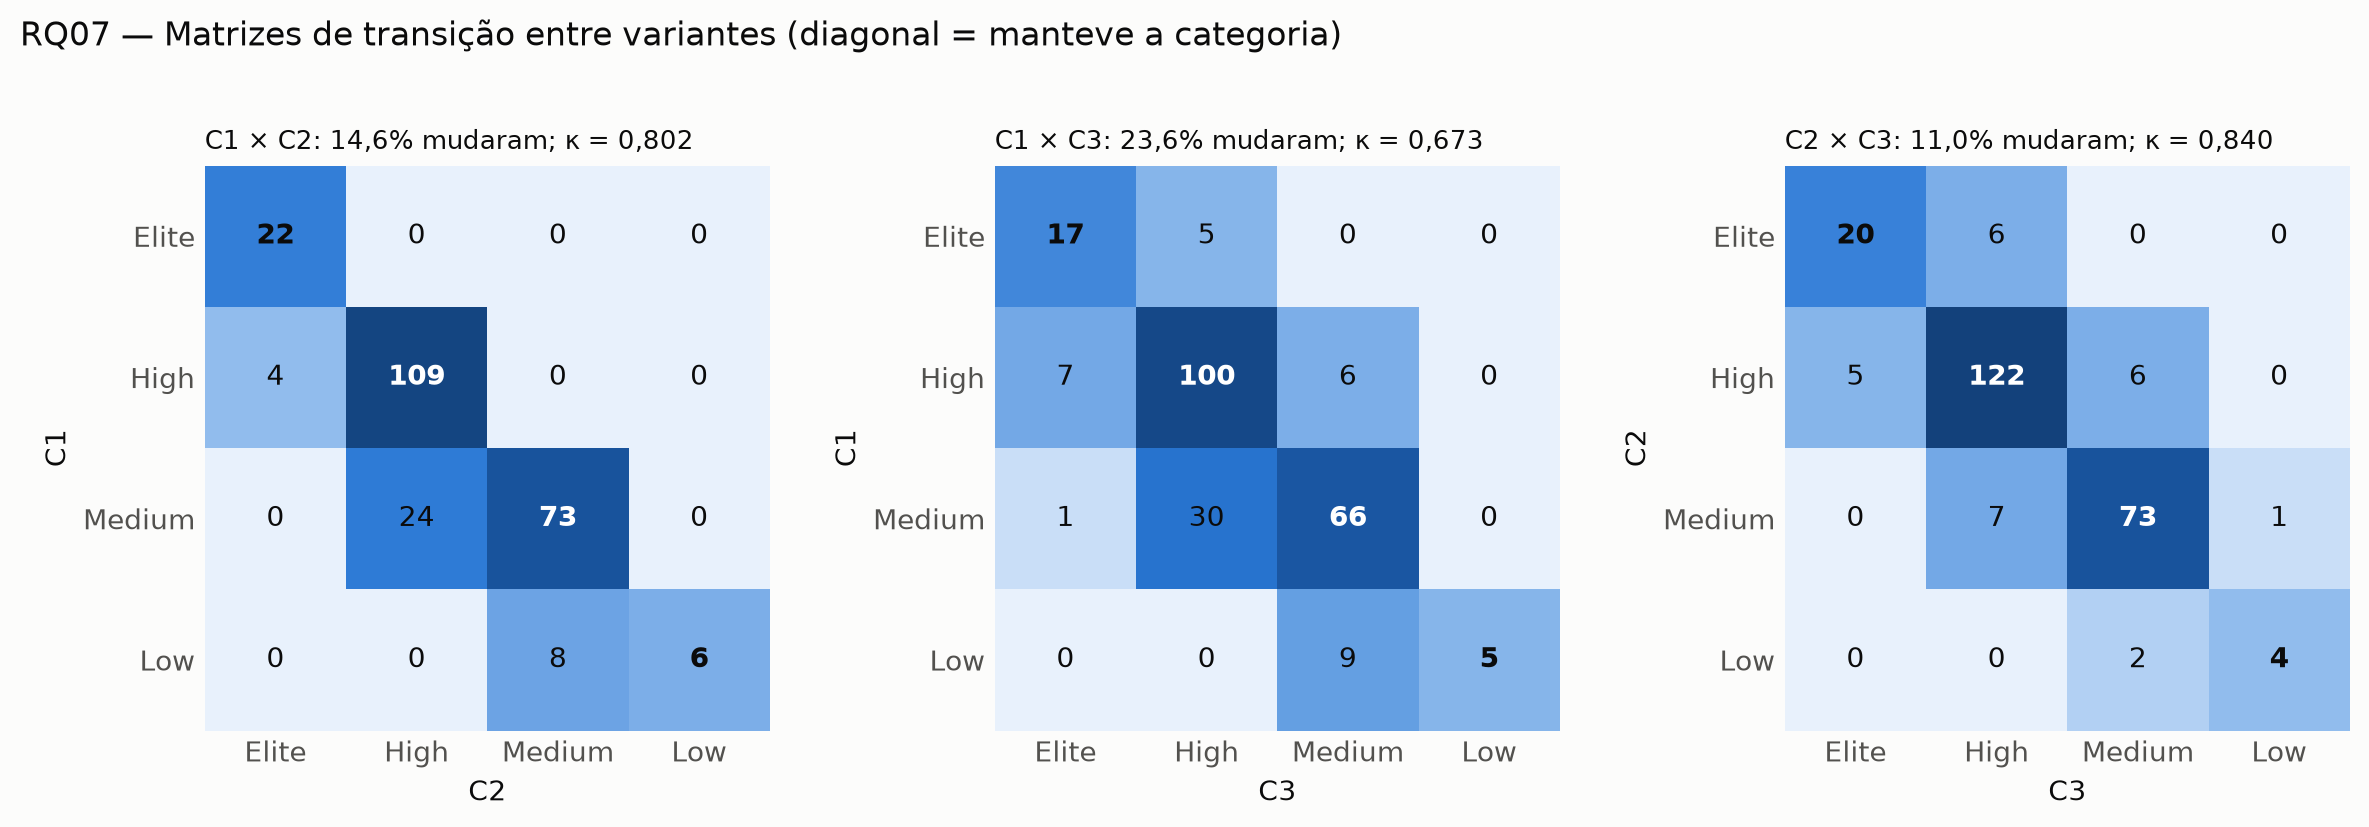
\includegraphics[width=0.82\textwidth]{fig10_rq07_transicoes.png}
  \caption{RQ07: matrizes de transição entre as variantes C1, C2 e C3.}
  \label{fig:rq07}
\end{figure}

\textbf{RQ08 (bônus).} O \emph{rework rate} mediano é de 0,769 (IQR
0,52--0,91), contra 0,429 do CFR (b) e 0,053 do CFR (a). Na escala
trimestral exigida, com 4 pontos por repositório, nenhum repositório tem
tendência significativa. Na escala mensal, 15,2\% aumentam a frequência de
deploy e 6,7\% a reduzem, e o CFR (a) cai em 7,3\% e sobe em 4,4\%
(Figura~\ref{fig:rq08}).

\begin{figure}[ht]
  \centering
  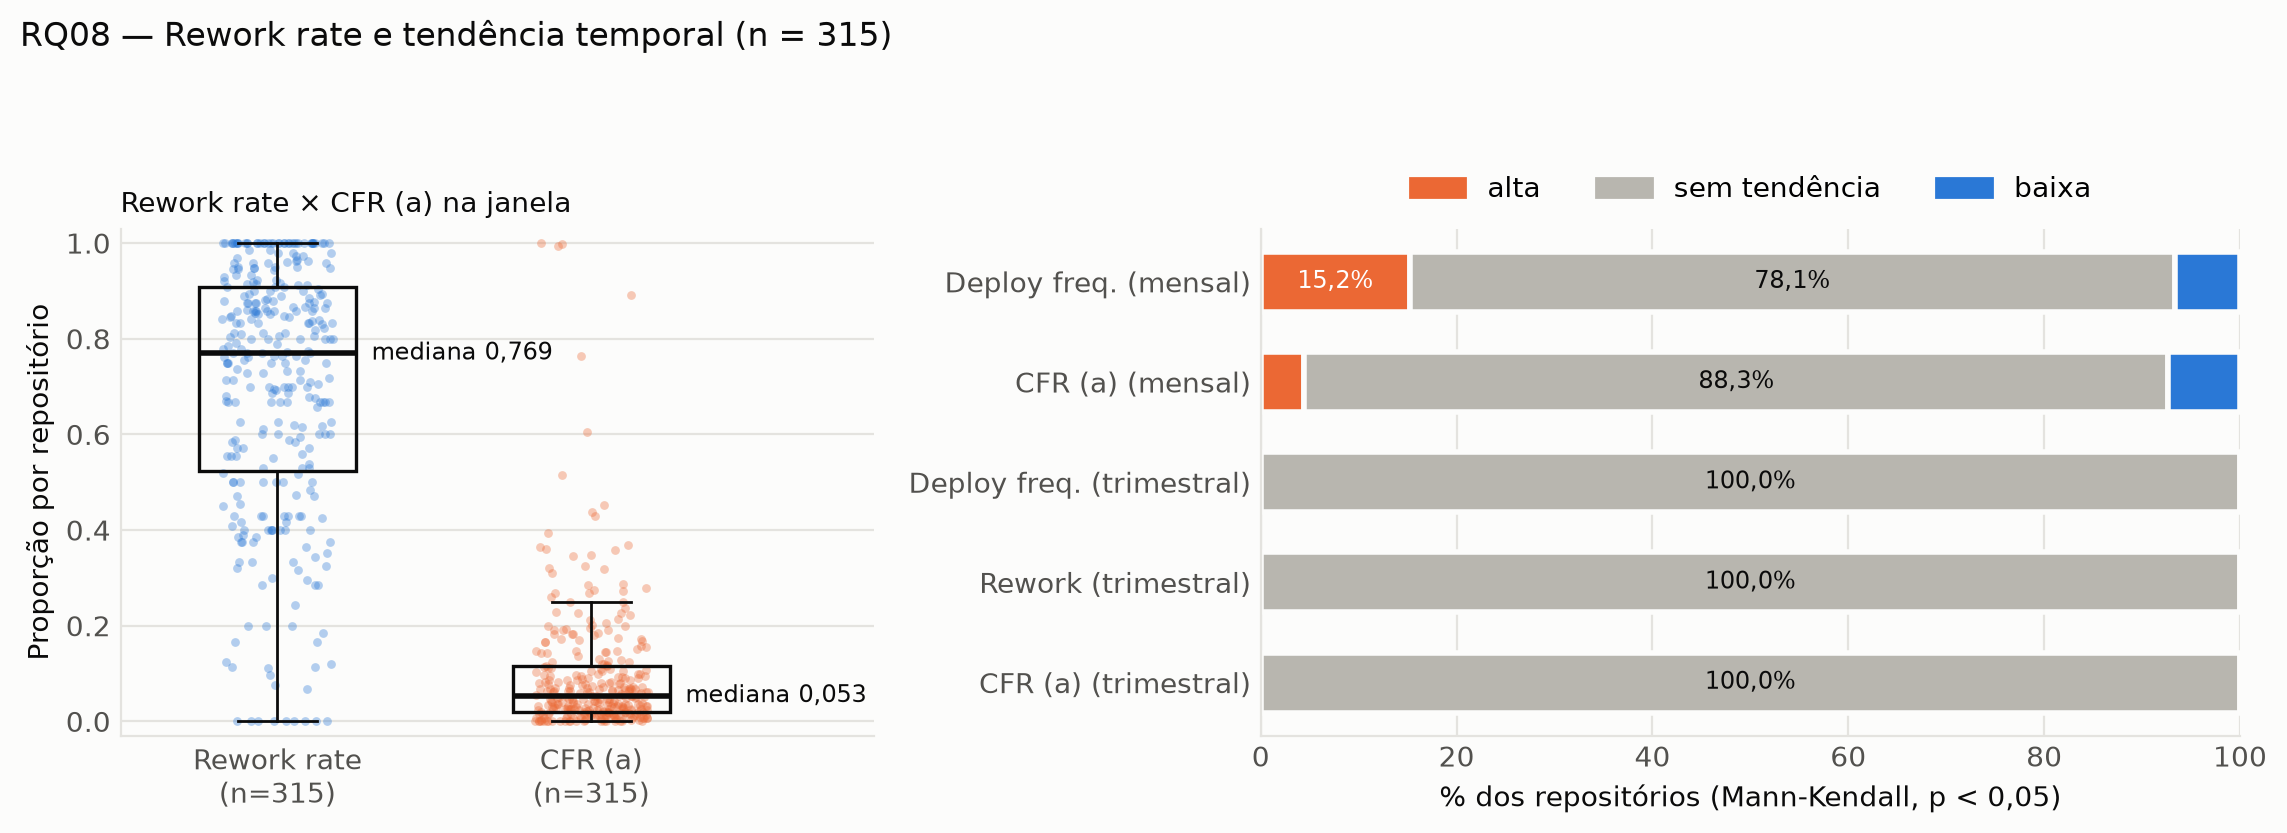
\includegraphics[width=0.82\textwidth]{fig11_rq08_rework_tendencia.png}
  \caption{RQ08: \emph{rework rate} e tendências de Mann-Kendall ($p < 0{,}05$).}
  \label{fig:rq08}
\end{figure}

% =====================================================================
\section{Discussão}

A Tabela~\ref{tab:hip} confronta as hipóteses com os resultados.

\begin{table}[ht]
  \centering
  \caption{Hipóteses informais $\times$ resultados.}
  \label{tab:hip}
  \small
  \begin{tabularx}{\textwidth}{lYl}
    \toprule
    RQ & Resultado & Veredito \\
    \midrule
    RQ01 & mediana 0,35/semana; 28\% abaixo de mensal; 3 diários & confirmada \\
    RQ02 & (a) 166~h $>$ (b) 152~h; (a) maior em 69\% dos repositórios & confirmada \\
    RQ03 & CFR (a) 5,3\% $<$ CFR (b) 42,9\%; heurística com precisão 0,44 e recall 0,84 & refutada \\
    RQ04 & $\rho$(runs, recuperação) = 0,01 & refutada \\
    RQ05 & $\rho = +0{,}13$ (a) e $+0{,}69$ (b) & refutada (sinal) \\
    RQ06 & tipo sem efeito; idade é o fator dominante & refutada \\
    RQ07 & Elite estável em C1 $\to$ C2; 8 de 14 Low sobem & confirmada \\
    RQ08 & mensal: mais melhoras que pioras; trimestral sem tendências & confirmada (mensal) \\
    \bottomrule
  \end{tabularx}
\end{table}

\textbf{Os proxies não são intercambiáveis.} O CFR (a) mede quebras de
pipeline, que os projetos corrigem rápido e em pequena proporção. O CFR (b)
tenta medir falhas que chegam ao usuário, mas depende de uma heurística com
muitos falsos positivos: 112 das 199 releases que ela marca como corretivas
não o são no consenso. Os 42,9\% são, portanto, um \textbf{limite superior}.
A classe é ambígua até para humanos ($\kappa = 0{,}60$), porque muitas
releases misturam correções e funcionalidades ou não têm notas. A diferença
entre as variantes de lead time confirma a pista do enunciado: a mediana por
release é puxada por commits antigos que esperam a próxima release, enquanto a
variante por commit dilui esses casos.

\textbf{Velocidade $\times$ estabilidade.} Ao contrário da afirmação do DORA
de que não há \emph{trade-off} \cite{forsgren2018}, aqui quem entrega mais
também falha mais. O efeito é fraco no CI e forte na entrega. Parte da
correlação em (b) é mecânica: com mais releases, cresce a chance de uma
release ser seguida por outra corretiva em até 7 dias, e a heurística
favorece versões de patch, que são justamente as mais frequentes. A RQ06
sugere um fator comum, a maturidade. Projetos jovens se comportam como
``startups'' (entregam mais, mais rápido, recuperam mais rápido e corrigem
mais), enquanto projetos maduros são lentos e estáveis. Dentro de cada
repositório, ao longo do ano, o padrão não se repete: entre os que mudam,
predominam os que aceleram e os que reduzem o CFR de CI (RQ08). Ou seja, a
correlação entre repositórios não indica que acelerar \emph{cause} mais
falhas.

\textbf{Robustez da classificação.} A classificação DORA é razoavelmente
robusta ($\kappa$ de 0,67 a 0,84), mas não neutra. Contar tags como deploy é
uma decisão sistemática: só melhora categorias, porque aumenta a frequência
sem afetar as outras métricas. Trocar o lead time por release pelo lead time
por commit muda quase um quarto das categorias e é a única troca que rebaixa
repositórios Elite. Comparações de ``nível DORA'' entre estudos, portanto, só
fazem sentido com a mesma definição operacional.

\textbf{O que as inovações acrescentaram.} O Kaplan-Meier mostrou que, com
1,1\% de censura, ignorar os episódios abertos não distorceria a recuperação
(4,4~h contra 3,3~h). Essa conclusão só é possível porque a censura foi
tratada. O \emph{post-hoc} de Dunn transformou ``a idade importa'' em um
padrão interpretável. A escala mensal do Mann-Kendall encontrou as tendências
que a escala trimestral, com só 4 pontos, não tem poder para detectar: mesmo
uma série perfeitamente monotônica dá $p \approx 0{,}09$.

% =====================================================================
\section{Ameaças à validade}

Seguimos as quatro categorias de validade de Wohlin et al.\ \cite{wohlin2012}. O detalhamento,
com evidências e mitigação de cada ameaça, está em \code{docs/threats.md}.

\textbf{Construto.} (i) Release não é deploy: bibliotecas publicam em
registries, e serviços podem implantar sem release. Contar tags mudou a
categoria de 14,6\% dos repositórios (RQ07). (ii) Os dois CFR são proxies, e
a heurística de release corretiva tem F1 = 0,57, o que infla o CFR (b) e o
\emph{rework rate}. (iii) A data de autoria do commit é distorcida por
\emph{rebase} e \emph{squash merge}, e 15,8\% das releases ficaram fora do
lead time por \code{compare} 404. (iv) A recuperação mede o CI, não o
restabelecimento de um serviço.

\textbf{Interna.} (i) A idade é um possível confundidor de linguagem e
frequência, e não houve controle multivariado: a RQ06 é associativa. (ii) Um
dos três avaliadores foi um modelo de linguagem, e a concordância foi só
moderada nas dimensões ``entrega'' e ``corretiva''. O gabarito, portanto,
também é imperfeito: um avaliador marcou 183 das 300 releases como
corretivas, contra 99 e 103 dos outros dois. (iii) A heurística foi escolhida
na mesma amostra em que foi avaliada; a validação cruzada mitiga, mas não
elimina, esse otimismo. (iv) Monorepos e releases automáticas inflam a
contagem de deploys.

\textbf{Externa.} A amostra cobre projetos open-source populares, ativos, com
releases formais e GitHub Actions. Os resultados não se generalizam para
times corporativos, para projetos com CI externa nem para quem implanta sem
releases. A janela é única, de 12 meses.

\textbf{Conclusão.} Os 20 testes da RQ06 foram corrigidos por Holm, e os
tamanhos de efeito separam significância de relevância. O fator tipo tem só
55 repositórios, o que traz risco de erro tipo II. Os 315 testes de
Mann-Kendall por métrica não foram corrigidos (cerca de 16 falsos positivos
esperados a 5\%), então as proporções mensais da RQ08 são indicativas. Toda a
análise é não paramétrica e não houve imputação de ausentes.

% =====================================================================
\section{Replicação cruzada}

Esta seção será completada na entrega final. O pipeline de outro grupo será
executado apenas pelo README sobre uma subamostra de 30 repositórios. Em
seguida, compararemos a diferença relativa por métrica e a porcentagem de
repositórios com a mesma classificação DORA, e abriremos Issues com as
divergências. Para o nosso próprio pipeline, o README oferece reprodução
exata, sem token, a partir do manifesto e dos JSONs versionados, e o script
\code{scripts/diff\_datasets.py} automatiza a comparação dos CSVs.

% =====================================================================
\section{Conclusão}

Os 315 repositórios populares que usam GitHub Actions entregam com cadência
moderada, levam cerca de uma semana do commit à release e se recuperam de
falhas de CI em poucas horas. A maioria fica nas categorias High e Medium. A
taxa de falha depende fortemente do proxy, e o proxy de entrega só é
utilizável como limite superior: mesmo após quatro versões e 197
combinações, a heurística de release corretiva não passou de F1 = 0,57, e os
próprios avaliadores concordaram apenas moderadamente. Entre repositórios,
velocidade e estabilidade aparecem como \emph{trade-off}, mediado pela idade
do projeto; dentro de cada repositório, ao longo do ano, as melhorias tendem
a vir juntas. A classificação DORA é robusta o suficiente para comparar
grupos, mas a definição operacional precisa acompanhar qualquer número
reportado.

Como trabalhos futuros, propomos:
\begin{itemize}
  \item classificar o texto das notas de release, e não só as mensagens de
    commit, para melhorar a heurística;
  \item usar fontes de deploy mais próximas da produção, como os
    \emph{deployments} do GitHub e as publicações em registries;
  \item ajustar um modelo multivariado que separe o efeito da idade dos
    demais fatores.
\end{itemize}

\medskip
\noindent\textbf{Repositório:}
\url{https://github.com/luisajardim/Lab-Experimentacao-e-Medicao-}
(pasta \code{Enunciado 3}).

\bibliographystyle{sbc}
\bibliography{referencias}

\end{document}
